%!TEX root = ../../prace.tex

\subsection{Bloky a~herní svět}
\label{subsec:bloky}

Pro naše potřeby bude stačit, když budeme mít bloky zarovnané do jednotné mřížky v~rámci celého světa (tedy tak, jak to má \MC{}). Z~toho vyplývá, že nebudeme požadovat implementaci volné počáteční rotace bloku (ve smyslu rotace kolem vertikální osy). Opět zdůrazňujeme, že budeme implementovat prototyp hry se stavěním různě velkých bloků, jednotná mřížka tudíž bude v~této fázi dostačovat. S~tím souvisí další zjednodušení -- nechceme řešit terén ani jeho modifikace a~s~tím související řešení umisťování bloků. V~této fázi si vystačíme s~pouhou rovinou. Protože hry z~kapitoly \ref{chap:uvod} mají rozsáhlé světy a~techniky implementace rozsáhlých světů nejsou úplně triviální (použití systému chunků, streamování levelů apod.), nevidíme jako přínosné se jimi zabývat, aniž bychom věděli, že samotná koncepce stavby dynamicky škálovatelných bloků je správný směr dalšího vývoje. Proto budeme pro účely této práce považovat celou herní mapu se všemi postavenými a~umístěnými objekty za dostatečně malou, která (ač celá načtená v~paměti) zásadním způsobem neovlivňuje výkon ani vykreslování hry. Samozřejmě budeme požadovat, aby i~v~této variantě byla implementace herního světa dostatečně efektivní jak z~pohledu výkonu, tak i~z~pohledu paměťové náročnosti. Podrobnější rozbor herního světa bude v~detailní analýze v~části \ref{sec:blocksWorld}.

Budeme chtít mít bloky, které nebudou pouze statické objekty ve hře. Bloky by měly mít svůj význam ve světě a~mělo by jít s~nimi interagovat. Navíc budeme chtít, aby bloky byly vizuálně přitažlivé, což bude u~některých bloků znamenat, že je budeme muset vymodelovat v~nějakém 3D modelovacím programu. \textit{Multiblokový} systém není potřeba implementovat. Vzhledem k~dynamickému škálování bloků bude potřeba vyřešit škálování textur v~rámci 3D modelů a~jejich UV mapování -- chceme, aby se textury chovaly \uv{inteligentně} a~při škálování bloku se textury (při zachování mapování na geometrii modelu) neroztahovaly do nějakých nepěkných výtvorů. 


Dále budeme chtít, aby bylo možné definovat jednotlivé vlastnosti bloků jednoduchým a~přímočarým způsobem, nejlépe mimo samotný zdrojový kód hry a~v~nějakém editoru. Tento požadavek je zde z~toho důvodu, že je zcela běžné, že herní designéři ladí různé konstanty a~nastavení během vývoje tak, aby hra co nejvíce odpovídala jejich představám a~byla pro hráče zábavná. Mít tedy tyto konstanty pevně zakompilované v~kódu by znamenalo opětovnou kompilaci celého projektu, což v~pozdějších fázích může znamenat výrazné zpomalení vývoje. Protože očekáváme další vývoj této hry, měli bychom se držet nějakých rozumných postupů na udržovatelnost kódu a~celého vývoje hry.

\subsubsection{Vlastnosti bloků}
\label{subsubsec:vlastnosti}

Chceme navrhnout systém, ve kterém bude nejmenší blok o~hraně 20 cm, tedy objemu odpovídajícímu 0,008 m$^3$. Tento blok nazveme jako \textit{jednotkový}, identicky s~tímto budeme používat i~pojem \textit{jednotková krychle}. Největší blok pak omezíme na 20-ti násobek jednotkové krychle ve všech 3 rozměrech. Největší blok tedy bude mít objem 64 m$^3$. Může se stát, že dolní limit bude příliš malý, ale v~tuto chvíli považujeme tuto konstantu za dostatečnou. Naopak horní limit bude nejspíše dostatečný -- práce s~příliš velkými bloky by mohla být neefektivní a~stavba nepřehledná.

V následující tabulce (tabulka \ref{table:requiredBlocks}) si popíšeme, jaké bloky budeme ve hře chtít mít, jak by měly vypadat a~co by měly umět. Bloky jsme rozdělili do dvou kategorií -- první (\textbf{A}) jsou \textit{konstrukční} prvky, druhá kategorie (\textbf{B}) obsahuje \textit{funkční} prvky. \textit{Název} bloku je zřejmý. Sloupce \textit{Min} a~\textit{Max} popisují velikost bloku jako násobky jednotkové krychle. Dále jsou v~tabulce sloupce \textit{Pitch} a~\textit{Roll}. Ty popisují to, zda je blok možné rotovat podle daných os. Správně bychom tu měli mít i~sloupec \textit{Yaw}, ale protože je pro všechny bloky povolen, tak jsme tento sloupec vynechali. Smysl rotací lze nahlédnout v~obrázku \ref{fig:axes}.

\begin{figure}[!ht]\centering
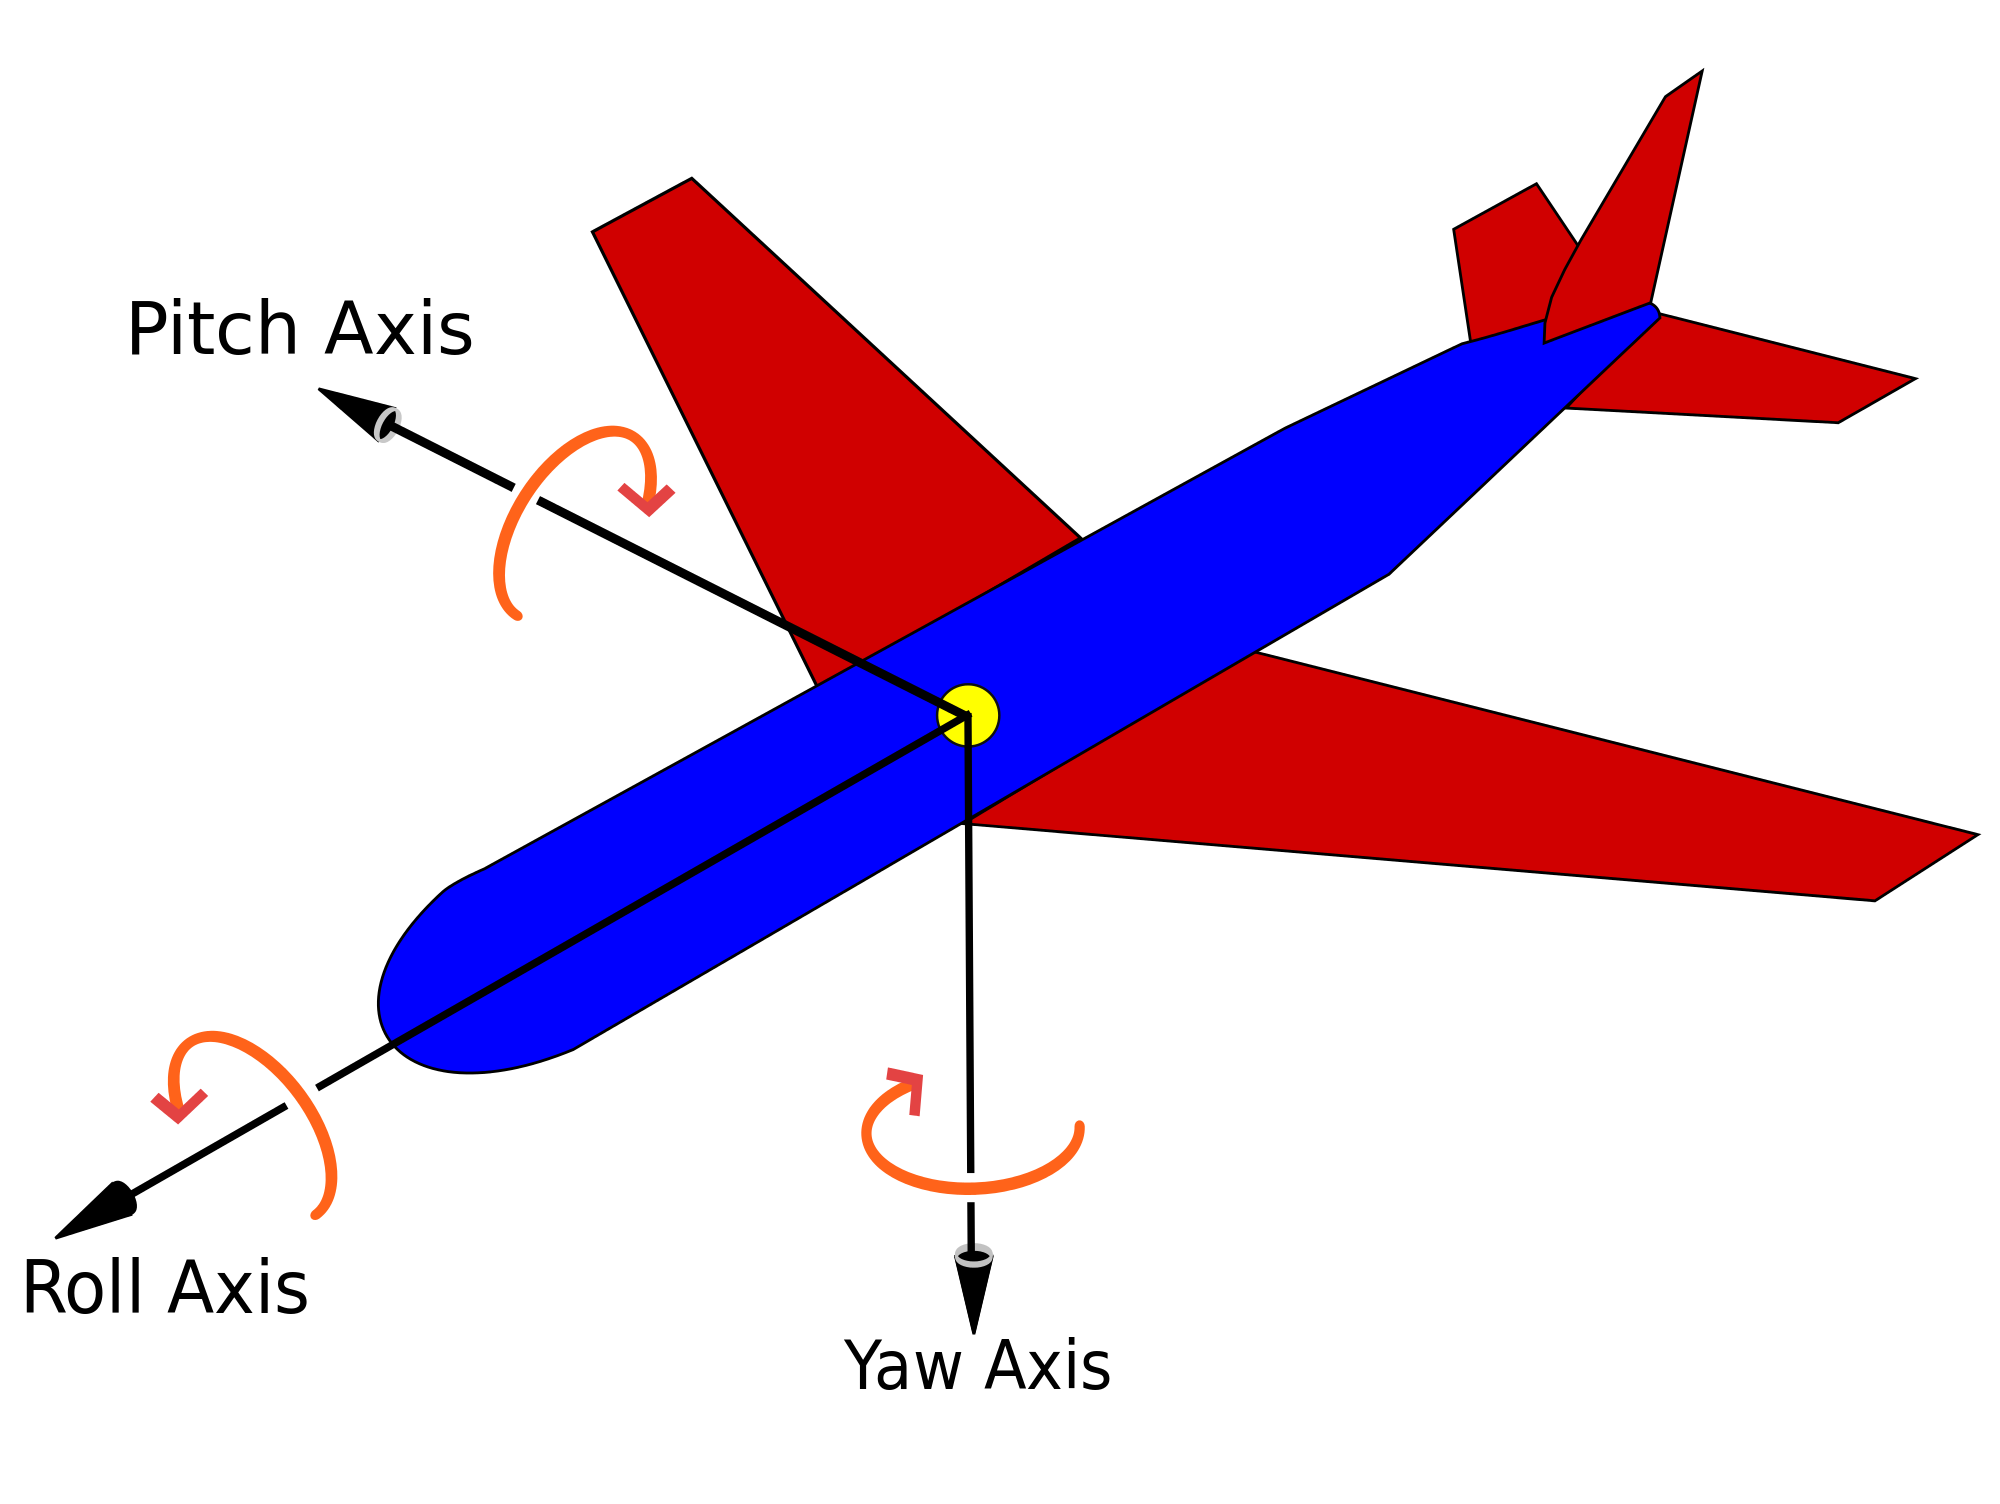
\includegraphics[ width=90mm]{../img/analysis/Yaw_Axis_Corrected}

\caption{Rotace modelované na letadle. Zdroj: en.wikipedia.org~\citep{wp_axes}}
\label{fig:axes}

\end{figure}



Jako poslední je sloupec \textit{T}, tedy typ bloku. Typ bloku může být: \textit{Kostka}, \textit{Zkosený}, \textit{Rohový}, \textit{Vlastní}. Typ pak ovlivňuje další vlastnosti bloku, jako například cenu za jeho postavení, ale i~jeho zdraví. Podrobnější popis, včetně algoritmu výpočtu, je v~části \ref{subsec:instVlast}.


\FloatBarrier


\begin{table}[h]
\begin{tabular}{|rll*{5}{c}|}
	\hline
	\tableColumnTitles{Název}								{	&	\rotatebox{0}{Min~} 		&	\rotatebox{0}{Max~}			&	\rotatebox{90}{Pitch~}			&	\rotatebox{90}{Roll~}			& \rotatebox{90}{Typ~}	}		\hline
	\currentCategory{\textbf{Základní bloky}} 																					\\		\hline
		\mytablerow 				& Blok základny				& 1--1--4	& 20--20--4		& 				& 				&K	\\		\hline
		\mytablerow 				& Blok stavby				& 1--1--1	& 20--20--20	& \checkmark	& \checkmark	&K	\\		\hline
		\mytablerow 				& Blok polykarbonátu		& 1--1--1	& 20--20--20	& \checkmark	& \checkmark	&K	\\		\hline
		\mytablerow 				& Zkosený blok základny		& 1--1--4	& 20--20--4		& 				& 				&Z	\\		\hline
		\mytablerow 				& Zkosený blok stavby		& 1--1--1	& 20--20--20	& \checkmark	& \checkmark	&Z	\\		\hline
		\mytablerow 				& Roh bloku stavby			& 1--1--1	& 20--20--20	& \checkmark	& \checkmark	&R	\\		\hline
	\currentCategory{\textbf{Speciální bloky}} 									 												\\		\hline
		\mytablerow 				& Terminál			 		& 1--8--5 	& 1--8--5		& 				& 				&V	\\		\hline
		\mytablerow 				& Napájené okno				& 2--1--2	& 20--1--20		& \checkmark	& \checkmark	&K	\\		\hline
		\mytablerow 				& Dveře 					& 7--7--11	& 7--7--11		& 				& 				&V	\\		\hline
		\mytablerow 				& Světlo					& 1--1--1	& 1--1--1		& \checkmark	& \checkmark	&V	\\		\hline
		\mytablerow 				& Přepínač 					& 1--1--1	& 1--1--1		& \checkmark	& \checkmark	&V	\\		\hline
		\mytablerow 				& Generátor energie			& 3--3--2	& 20--20--2		& 				& 				&K	\\		\hline
		\mytablerow 				& Generátor objektů 		& 3--3--2	& 20--20--2		& 				& 				&K	\\		\hline
		\mytablerow 				& Akumulátor				& 3--3--3	& 3--3--3		& 				& 				&V	\\		\hline
		\mytablerow 				& Plnička kyslíkových bomb 	& 4--3--4	& 4--3--4		& 				& 				&V	\\		\hline
		\mytablerow 				& Kyslíková bomba			& 2--2--2	& 2--2--2		& 				& 				&V	\\		\hline
		
\end{tabular}
\caption{Požadované bloky a~jejich základní vlastnosti}
\label{table:requiredBlocks}
\end{table}

\FloatBarrier


\subsection{Podrobný popis bloků}

V následujících odstavcích si podrobně popíšeme všechny bloky a~nastíníme jejich význam. Některé bloky mohou obsahovat elektrické a~kyslíkové \textit{komponenty}. Význam těchto komponent a~důvod, proč je budeme chtít mít jako komponenty bude řešen v~části \ref{sec:komponents}.



\subsubsection{A1 -- Blok základny}
\label{blocks:A1}
Tento blok je ve hře z~toho důvodu, protože má sloužit jako základový blok staveb. Pokud bychom měli nerovný terén, tento blok by mohl zahrnovat podstavce pro vyrovnání terénu. Velikost v~ose Z~je omezena na 4 základní bloky. Obsahuje \textit{elektrickou komponentu}.


\subsubsection{A2 -- Blok stavby}
\label{blocks:A2}
Tento blok je základním stavebním blokem ve hře, a~proto může existovat ve všech možných velikostech. Obsahuje \textit{elektrickou komponentu}.


\subsubsection{A3 -- Blok polykarbonátu}
\label{blocks:A3}
Tento blok je nejlevnější, neobsahuje žádné komponenty. Ideou bloku je podpora průhledných stěn a~také možné pomocné stavební konstrukce pro výstavbu do výšky. Inspiraci můžeme vidět v~používání třeba bloku hlíny ve hře \MC{}, kdy hráč vyskočí a~pod sebe umístí nový blok hlíny, a~tím se ve světě posune o~1~metr výš.


\subsubsection{A4 -- Zkosený blok základny}
\label{blocks:A4}
Tento blok je zde ze stejného důvodu jako blok \RB{A1}. Má stejné vlastnosti, pouze má zkosený tvar. Může sloužit jako přístupová rampa.


\subsubsection{A5 -- Zkosený blok stavby}
\label{blocks:A5}
Obdobně jako u~základny, tento blok má stejné vlastnosti jako \RB{A2}, pouze má jiný tvar.


\subsubsection{A6 -- Roh bloku stavby}
\label{blocks:A6}
Tento blok má stejné vlastnosti jako \RB{A2} a~opět definuje pouze jiný tvar.



\subsubsection{B1 -- Terminál}
\label{blocks:B1}
Terminál má pevnou velikost (1 x 8 x 5 bloků) a~měl by vypadat jako nějaká obrazovka budoucnosti. Obsahuje \textit{elektrickou komponentu}. Terminál by pro hráče měl být použitelný přímo i~nepřímo. Přímé použití by mělo dobít herní postavě energii, nepřímé by mělo otevřít uživatelské rozhraní.

\subsubsection{B2 -- Napájené okno}
\label{blocks:B2}
Napájené okno je omezeno pouze v~jednom rozměru, jinak povolíme velikost od 2 do 20 násobku jednotkové krychle. Dolní omezení je zde z~toho důvodu, že okno o~velikosti 20 x 20 cm je zbytečně malé. Obsahuje \textit{elektrickou komponentu}.


\subsubsection{B3 -- Dveře}
\label{blocks:B3}
Dveře jsou další ze speciálních bloků s~pevnou velikostí (7 x 7 x 11 bloků). Jejich účel je jasný -- možnost uzavření budovy a~pokud se rozhodneme implementovat systém okysličování vnitřků budov, tak i~hermetické uzavření jednotlivých místností.


\subsubsection{B4 -- Světlo}
\label{blocks:B4}
Blok světla má také jasný účel -- osvětlení míst, kde není dostatek přirozeného světla či osvětlení v~budově, pokud nastane noc. Světlo by mělo být možné použít (přinejmenším ho chceme umět vypnout a~zapnout). Obsahuje \textit{elektrickou komponentu}. 


\subsubsection{B5 -- Přepínač}
\label{blocks:B5}
Účel přepínače je zřejmý -- ovládání ostatních bloků. Proto bude muset být použitelný. Skvělé by bylo, kdybychom na základě vizualizace modelu přepínače ihned poznali stav, ve kterém se přepínač nachází. Obsahuje \textit{elektrickou komponentu}. 


\subsubsection{B6 -- Generátor energie}
\label{blocks:B6}
Tento blok byl přidán proto, aby hráč získával novou elektrickou energii z~prostředí. Energie je vyráběna během bouře kyselého deště (více o~kyselém dešti v~části \ref{subsubsec:weather}), tato mechanika bude podrobněji popsána později. Na výšku byl blok omezen na 2 jednotkové krychle. Obsahuje \textit{elektrickou komponentu}. 


\subsubsection{B7 -- Generátor objektů}
\label{blocks:B7}
Smyslem tohoto bloku je generování nových bloků. Vzhledem k~dalším herním mechanikám můžeme říct, že to je spíše nutná komponenta \textit{Konstruktoru objektů} (sekce \ref{sec:konstruktor}). Na výšku byl blok omezen na 2 jednotkové krychle. Obsahuje \textit{elektrickou komponentu}.


\subsubsection{B8 -- Akumulátor}
\label{blocks:B8}
Tento blok byl do hry přidán z~toho důvodu, že je potřeba pokrýt elektrické nároky stavby v~období, kdy neprší kyselý déšť. Funkce akumulátoru je tedy uchování elektrické energie. Z~toho vyplývá, že musí obsahovat \textit{elektrickou komponentu}. Bylo by také hezké, kdybychom měli ve hře rychlý náhled na úroveň jeho nabití.


\subsubsection{B9 -- Plnička kyslíkových bomb}
\label{blocks:B9}
Plnička je příklad bloku, který má \textit{elektrickou} a~zároveň \textit{kyslíkovou komponentu}. Jejím cílem je plnit Kyslíkové bomby kyslíkem. Zároveň by bylo hezké, kdyby blok uměl doplnit kyslík herní postavě napřímo. Pokud to bude možné, rádi bychom viděli (podobně jako u~stolu v~\ME{}) náhled plněné kyslíkové bomby. Tedy aby hráč na první pohled věděl, zda je nějaká bomba plněna.

\subsubsection{B10 -- Kyslíková bomba}
\label{blocks:B10}
Tento blok slouží k~uchování kyslíku, použitím tohoto bloku je možné doplnit kyslík herní postavě. Zároveň je možné tento blok sebrat do inventáře a~později z~inventáře umístit do herního světa. Má \textit{kyslíkovou komponentu}. Pokud to bude možné, chtěli bychom hráči zobrazit stav naplnění, stejně jako u~\RB{B8}.


